%!TEX TS-program = xelatex
%!TEX encoding = UTF-8 Unicode
% Awesome CV LaTeX Template for CV/Resume
%
% This template has been downloaded from:
% https://github.com/posquit0/Awesome-CV
%
% Author:
% Claud D. Park <posquit0.bj@gmail.com>
% http://www.posquit0.com
%
% Template license:
% CC BY-SA 4.0 (https://creativecommons.org/licenses/by-sa/4.0/)
%
%-------------------------------------------------------------------------------
% CONFIGURATIONS
%-------------------------------------------------------------------------------
% A4 = a4paper, Letter = letterpaper
\documentclass[12pt, a4paper]{awesome-cv}

% Default page margins:
% \geometry{left=1.4cm, top=.8cm, right=1.4cm, bottom=1.8cm, footskip=.5cm}

\geometry{left=1.5cm, top=.75cm, right=1.25cm, bottom=1.5cm, footskip=.5cm}

% Specify the location of the included fonts
\fontdir[fonts/]

% Color for highlights
% Awesome Colors: awesome-emerald, awesome-skyblue, awesome-red, awesome-pink, awesome-orange
%                 awesome-nephritis, awesome-concrete, awesome-darknight

% Custom Awesome Colors: awesome-midnight, awesome-lunar, awesome-sapphire, awesome-blue,
%						 awesome-deepemerald, awesome-pitchblack
\colorlet{awesome}{awesome-midnight}

% Colors for text
% Uncomment if you would like to specify your own color
% \definecolor{darktext}{HTML}{414141}
% \definecolor{text}{HTML}{333333}
% \definecolor{graytext}{HTML}{5D5D5D}
% \definecolor{lighttext}{HTML}{999999}

\definecolor{darktext}{HTML}{111111}
\definecolor{text}{HTML}{111111}
\definecolor{graytext}{HTML}{111111}
\definecolor{lighttext}{HTML}{111111}

% Set false if you don't want to highlight section with awesome color
\setbool{acvSectionColorHighlight}{true}
\setbool{acvEntryHighlight}{false}
\setbool{acvPositionHighlight}{true}


% If you would like to change the social information separator from a pipe (|) to something else
\renewcommand{\acvHeaderSocialSep}{\quad\textbar\quad}


%-------------------------------------------------------------------------------
%	PERSONAL INFORMATION
%	Comment any of the lines below if they are not required
%-------------------------------------------------------------------------------
% Available options: circle|rectangle,edge/noedge,left/right
% \photo[rectangle,edge,right]{./examples/profile}
\name{Kyle Patrick}{Salitrik}
\position{Programmer{\enskip\cdotp\enskip}Electromechanical Engineer}
\address{ADDRESS}
\mobile{+(00)000-000-0000}
\email{xxxxxxxxx@gmail.com}
%\homepage{}
\github{NullFragment}
\linkedin{ksalitrik}
% \gitlab{gitlab-id}
\stackoverflow{789504}{NullFragment}


%-------------------------------------------------------------------------------
%	LETTER INFORMATION
%	All of the below lines must be filled out
%-------------------------------------------------------------------------------
% The company being applied to
\recipient
  {Company}
  {Address \\ Address \vspace{-3em}}
% The date on the letter, default is the date of compilation
\letterdate{}
% The title of the letter
\lettertitle{Job Application for Position}
% How the letter is opened
\letteropening{To Whom It May Concern,\vspace{-1em}}
% How the letter is closed
\letterclosing{Sincerely,}
% Any enclosures with the letter
%\letterenclosure[Attached]{Résumé}


\usepackage{float,outlines,hyperref}
\hypersetup{colorlinks=true,urlcolor=awesome-midnight}
%-------------------------------------------------------------------------------
\begin{document}

% Print the header with above personal informations
% Give optional argument to change alignment(C: center, L: left, R: right)
%\makecvheader[C]
\vspace{-1em}
% Print the footer with 3 arguments(<left>, <center>, <right>)
% Leave any of these blank if they are not needed
\makecvfooter
  {}
  {Kyle P. Salitrik~~~·~~~Portfolio Reference}
  {}

% Print the title with above letter informations
% \makelettertitle

%-------------------------------------------------------------------------------
%	LETTER CONTENT
%-------------------------------------------------------------------------------
\begin{cvletter}

\lettersection{New Hearthstone Card}
\quad 

\begin{figure}[H]
	\centering
	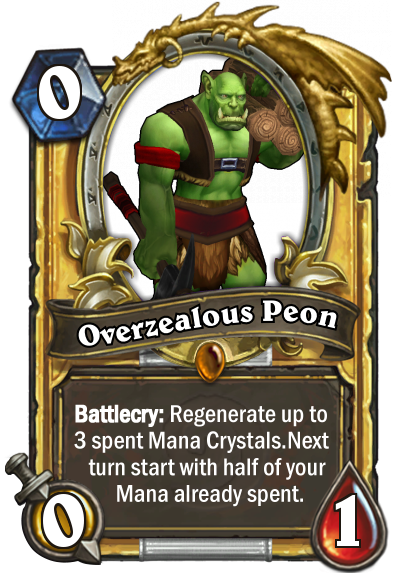
\includegraphics[scale=.6]{card.png}
\end{figure}
The reason that I believe this card would be an interesting fit (at least in Wild play) is because it can be used in low-risk, low-reward or high-risk, high-reward situations. In the early game, using this card to play two 2 Mana cost cards on your second turn could leave you at a slight advantage, but incapacitate your for a single turn. In contrast if a player was at a severe disadvantage in the late game, playing this card could close the gap between the two players and potentially allow that person to win, at the cost of not being able to play any high-cost cards in the following turn.


Card artwork was obtained from here:
\url{http://www.moddb.com/mods/wc3r/images/peon-animations}\\
Card was generated from here: 
\url{http://www.hearthcards.net/}

\lettersection{My~ Portfolio}

For my game design portfolio, please refer to my GitHub repository: https://github.com/NullFragment
These repositories/directories specifically include game design work:\vspace{-1em}
\begin{outline}
	\1 \url{https://github.com/NullFragment/PSU_Class_Projects/tree/master/GAME_220}\vspace{-1em}
	\1 \url{https://github.com/NullFragment/PSU_Class_Projects/tree/master/GAME_250}\vspace{-1em}
	\1 \url{https://github.com/NullFragment/PSU_Class_Projects/tree/master/GAME_251}\vspace{-1em}
	\1 \url{https://github.com/NullFragment/OculusDrift}\vspace{-1em}
\end{outline}

The following is a small HTML5/JavaScript game created for class using the Construct2 Engine:\vspace{-1em}
\begin{outline}
	\1 \url{https://nullfragment.github.io/Ricoshot/}
\end{outline}

\end{cvletter}


%-------------------------------------------------------------------------------
% Print the signature and enclosures with above letter informations
%\makeletterclosing

\end{document}